% Compile twice with pdfLaTeX. The bibliography is included below.
\documentclass[conference,letterpaper]{IEEEtran}
\pdfminorversion=7
\usepackage[T1]{fontenc}
\usepackage[utf8]{inputenc}
\usepackage[english]{babel}
\usepackage{amsmath,amssymb}
\usepackage{graphicx,booktabs,array}
\usepackage{cite,url}
\usepackage{tikz}
\usetikzlibrary{arrows.meta,positioning}
\usepackage{float}
\usepackage[section]{placeins}
\usepackage{microtype}
\usepackage[hidelinks]{hyperref}

% The folder fig must be beside this .tex file.
\graphicspath{{fig/}}
\newcommand{\Ohm}{\Omega}
\newcommand{\kohm}{\mathrm{k}\Omega}
\newcommand{\uF}{\mu\mathrm{F}}
\newcommand{\nF}{\mathrm{nF}}
\newcommand{\V}{\mathrm{V}}
\newcommand{\A}{\mathrm{A}}
\newcommand{\W}{\mathrm{W}}
\newcommand{\Hz}{\mathrm{Hz}}
\newcommand{\kHz}{\mathrm{kHz}}
\tikzset{
    blk/.style={draw,rectangle,align=center,
        font=\footnotesize,minimum height=10mm,
        text width=21mm,inner sep=3pt},
    arr/.style={-{Latex[length=1.7mm]},line width=.5pt},
    aux/.style={blk,dashed}
}
\setlength{\tabcolsep}{3.5pt}
\renewcommand{\arraystretch}{1.12}

\title{Discrete Electronics Project: Class AB Audio Amplifier\\
Design and Simulation Report}
\author{
\IEEEauthorblockN{
María Fernanda Morales Calderón, Ian José Álvarez Arrieta,\\
Oscar Felipe Montejo Cordero, Bryan Alessandro Elizondo Fallas,\\
Andrés Obregón López}
\IEEEauthorblockA{
School of Electronics Engineering\\
Tecnológico de Costa Rica (TEC)\\
Analog One}
}

\begin{document}
\maketitle

\begin{abstract}
This paper presents the design and simulation of a discrete-component
Class AB audio amplifier developed by Analog One. The system combines
signal conditioning, voltage amplification, and a power stage to drive
an $8\,\Ohm$ loudspeaker. The design uses commercial component values
and considers signal quality, transistor bias, and heat dissipation.
The main calculations establish a $20\,\W$ output reference. In the
reported power-stage test, a $20\,\V$ peak input at $10\,\kHz$
produces $22.8\,\W$ of average load power. Calculated requirements
and simulation readings are presented in separate tables to support
a clear assessment of the design.
\end{abstract}
\begin{IEEEkeywords}
Class AB, audio amplifier, discrete circuits, MOSFET, circuit simulation.
\end{IEEEkeywords}

\section{Project Description}

The project develops an audio amplifier that increases the level of an
incoming audio signal and supplies the power needed by an $8\,\Ohm$
loudspeaker. Developed by Analog One, the design aims to reproduce the
signal at a useful output level while limiting distortion and power
losses.

The amplifier contains three stages. The preamplifier conditions the
incoming signal, the voltage amplifier increases its amplitude, and the
power stage provides the current required by the loudspeaker. The
Class AB output arrangement uses two complementary transistors that
share the audio waveform. A small resting current helps smooth the
transition between the positive and negative portions of the signal.

The design combines calculations, commercial component values, and
circuit simulation. The evaluation considers output power, signal
transfer, bias adjustment, and heat dissipation, together with the
interaction between the stages.

\section{Block Diagrams}
\subsection{Overall Amplifier}

Figure~\ref{fig:overall} shows how the signal moves through the
amplifier. Each stage has a specific role, from preparing the incoming
signal to delivering power to the loudspeaker.

\begin{figure}[H]
\centering
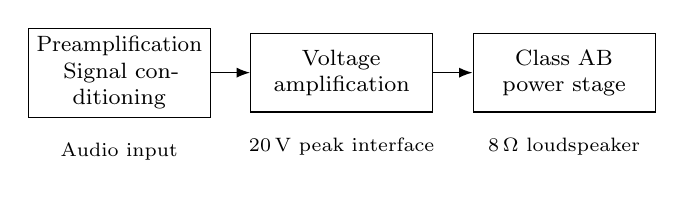
\begin{tikzpicture}[node distance=5mm]
\node[blk] (pre) {Preamplification\\Signal conditioning};
\node[blk,right=of pre] (gain) {Voltage\\amplification};
\node[blk,right=of gain] (power) {Class AB\\power stage};
\draw[arr] (pre)--(gain);
\draw[arr] (gain)--(power);
\node[below=2mm of pre,font=\scriptsize] {Audio input};
\node[below=2mm of gain,font=\scriptsize] {$20\,\V$ peak interface};
\node[below=2mm of power,font=\scriptsize] {$8\,\Ohm$ loudspeaker};
\end{tikzpicture}
\caption{Main stages of the audio amplifier.}
\label{fig:overall}
\end{figure}
\FloatBarrier

\subsection{Preamplification Stage}

\subsection{Voltage Amplification Stage}

\subsection{Class AB Power Stage}

The power stage uses an IRFZ44N and an IRF4905 MOSFET. These are
complementary transistors: one provides most of the current during the
positive portion of the signal, while the other handles most of the
negative portion. Class AB bias keeps both slightly conducting around
the transition, helping reduce crossover distortion
\cite[sec.~7--2]{floyd}.

The stage mainly increases the available current. Its output voltage
follows the input with the same polarity and a small reduction in
amplitude, as expected from a source-follower arrangement
\cite[sec.~9--2]{floyd}.

\begin{figure}[H]
\centering
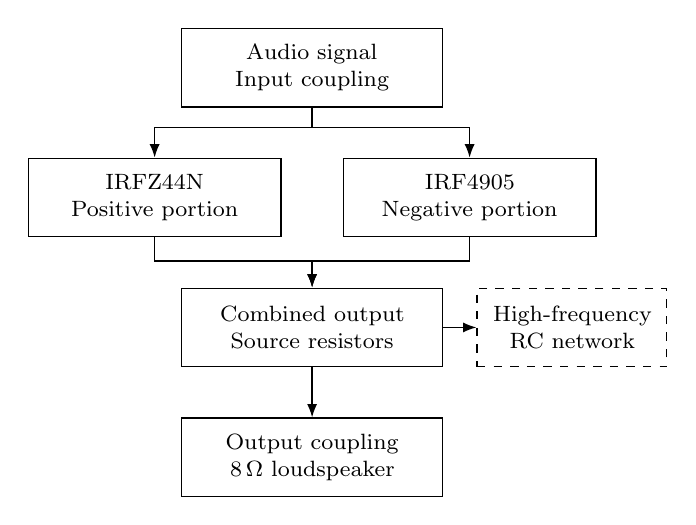
\begin{tikzpicture}
\node[blk,text width=31mm] (input) at (0,0)
    {Audio signal\\Input coupling};
\node[blk,text width=30mm] (n) at (-2,-1.65)
    {IRFZ44N\\Positive portion};
\node[blk,text width=30mm] (p) at (2,-1.65)
    {IRF4905\\Negative portion};
\node[blk,text width=31mm] (sum) at (0,-3.3)
    {Combined output\\Source resistors};
\node[blk,text width=31mm] (speaker) at (0,-4.95)
    {Output coupling\\$8\,\Ohm$ loudspeaker};
\node[aux,text width=22mm] (z) at (3.3,-3.3)
    {High-frequency\\RC network};
\draw[arr] (input.south)--++(0,-.25)-|(n.north);
\draw[arr] (input.south)--++(0,-.25)-|(p.north);
\draw[arr] (n.south)--++(0,-.3)-|(sum.north);
\draw[arr] (p.south)--++(0,-.3)-|(sum.north);
\draw[arr] (sum)--(speaker);
\draw[arr] (sum)--(z);
\end{tikzpicture}
\caption{Functional blocks of the Class AB power stage. The RC
network combines a resistor and a capacitor.}
\label{fig:powerblock}
\end{figure}
\FloatBarrier

\section{Design Considerations and Calculated Values}
\subsection{Preamplification Stage}

\subsection{Voltage Amplification Stage}

%%%%%%%%%%%%%%%%%%%%%%%%%%%%%%%%%%%%%%%%%%%%%%%%%%%%%%%%%%%%%%%%%%%%%%%%%%%%%%%%%%%%%%%%%%%%%%%%%%%%%%%%%%%%%%%%%%%%%%%%%%%%%%%%%%%%%%%%%%%%%%%%%%%%%%%%%%%%%%%%%%%%%%%%%%%%%%%%%%%%%%%%%%%%%%%%%%%%%%%%%%%%%%%
\subsection{Class AB Power Stage}

Figure~\ref{fig:schematic} presents the power-stage circuit. The design
retains the complementary output arrangement, with nominal supplies
of $+24\,\V$ and $-24\,\V$.

\begin{figure}[H]
\centering
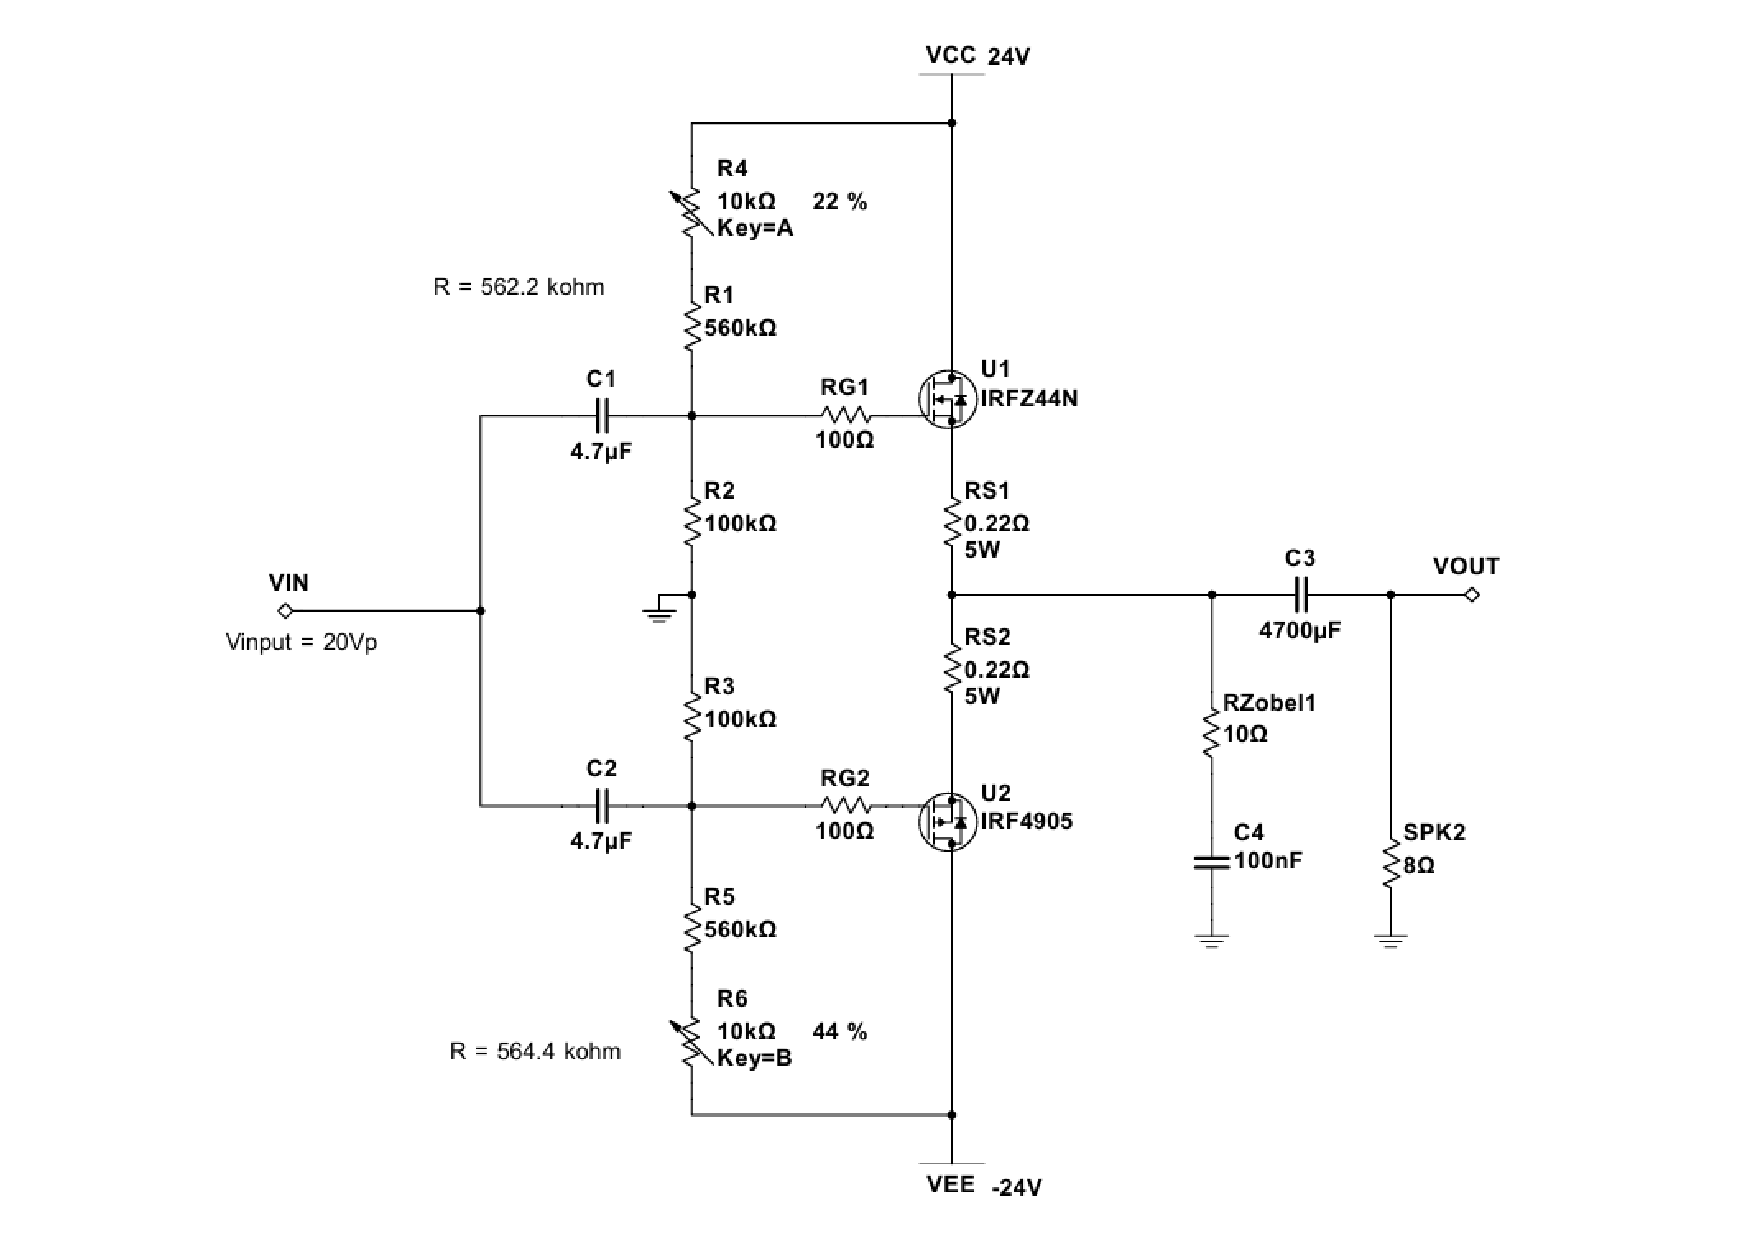
\includegraphics[width=\columnwidth,
    trim=95bp 10bp 110bp 15bp,clip]{pot20w.pdf}
\caption{Class AB power-stage schematic with IRFZ44N and IRF4905
MOSFETs.}
\label{fig:schematic}
\end{figure}
\FloatBarrier

\subsubsection{Output Power Requirement}


The design reference is $20\,\W$ delivered to an $8\,\Ohm$ load.
For a sinusoidal signal, the average power is
\begin{equation}
P_L=\frac{V_{L,\mathrm{rms}}^2}{R_L}.
\label{eq:power}
\end{equation}

Here, RMS is the effective voltage value used to calculate average
power of a signal audio. For this project the required voltage and current of this signal is:

\begin{align}
V_{LOAD,\mathrm{rms}}&=\sqrt{(20)(8)}\approx12.65\,\V,\\
V_{LOAD,peak}&=\sqrt{2}(12.65)\approx17.89\,\V,\\
I_{LOAD,\mathrm{rms}}&=\frac{12.65}{8}\approx1.58\,\A.
\end{align}

These values define the load requirements. With the specified
$20\,\V$ peak input, the output power depends on the voltage transfer
of the stage. Table~\ref{tab:loadcalc} summarizes the calculated values.

\begin{table}[!htb]
\caption{Calculated Output Requirements for the $20\,\W$ Reference}
\label{tab:loadcalc}
\centering\footnotesize
\begin{tabular}{@{}p{.61\columnwidth}p{.34\columnwidth}@{}}
\toprule
Quantity & Calculated value\\
\midrule
Average output power, reference & $20\,\W$\\
Load RMS voltage & $12.65\,\V$\\
Load peak voltage & $17.89\,\V$\\
Load peak-to-peak voltage & $35.78\,\V$\\
Load RMS current & $1.58\,\A$\\
Load peak current & $2.24\,\A$\\
\bottomrule
\end{tabular}
\end{table}
\FloatBarrier

\subsubsection{Class AB Bias Adjustment}

Bias sets the transistor operating conditions before an audio signal
is applied. The design adopts a resting-current target of
$I_D=50\,\mathrm{mA}$ in each branch. This resting-current is established to keep on the transistors in a operating point to represent always all the audio signal variations.

This small current provides
the intended overlap between the two transistors near the signal
transition \cite[sec.~7--2]{floyd}.

The $0.22\,\Ohm$ source resistors help control branch current and
provide a simple reference for adjustment. At the selected target,
the voltage across each resistor is
\begin{equation}
V_{RS,Q}=I_QR_S=(0.50)(0.22)=11\,\mathrm{mV}.
\end{equation}
The internal output is centered close to $0\,\V$ DC under this condition. To ensure the load (Speaker) only receives the audio signal.

The gate voltages are set by resistor dividers. For the resistor
connected toward either supply rail, its effective value follows a voltage divider:


\begin{equation}
R_{\mathrm{bias}}=100\,\kohm
\left(\frac{24\,\V}{|V_G|}-1\right)
\end{equation}


Using nominal gate settings of $+3.6243\,\V$ and $-3.6123\,\V$
gives effective resistances of $562.2\,\kohm$ and $564.4\,\kohm$.
Each branch therefore uses a commercial $560\,\kohm$ resistor in
series with a $10\,\kohm$ trimmer. The effective trimmer settings
are $2.2\,\kohm$ and $4.4\,\kohm$, corresponding to $22\%$ and
$44\%$ of their nominal range.

The gate settings provide the initial bias references. The resting
current is assessed through the source-resistor voltage drops.
Table~\ref{tab:biascalc} keeps these design references separate from
the recorded signal measurements.

\subsubsection{Signal Coupling}

The signal coupling is a factor to consider to keep isolated each stage of DC signals of polarization. Achieving that C1 and C2 pass the audio signal to the transistor gates while keeping their DC bias settings separate from the preceding stage.


This places the output coupling-network corner below $20\,\Hz$,
helping preserve low-frequency audio.

\subsubsection{Heat Dissipation}
For the Class AB configuration when it always be  bias also produces heat when no audio signal is present.
At the selected resting-current target, each transistor dissipates
approximately
\begin{equation}
P_{D,Q}\simeq V_{CC}I_Q=(24)(0.100)=2.40\,\W.
\end{equation}
During audio operation, dissipation is evaluated from the average
power absorbed by each transistor, including the overlapping conduction
of the Class AB stage.

A $10\,\W$ thermal design allowance per transistor provides margin
above the recorded losses of $6.58\,\W$ and $6.63\,\W$. The
heat-sink selection uses a thermal resistance of no more than
$4\,{}^\circ\mathrm{C/W}$ per device. A lower thermal resistance
allows heat to leave the transistor more easily. The selection also considers the device thermal data provided in
the transistor datasheets \cite{irfz44n,irf4905}.

\begin{table}[!htb]
\caption{Calculated Bias and Coupling Design References}
\label{tab:biascalc}
\centering\footnotesize
\begin{tabular}{@{}p{.61\columnwidth}p{.34\columnwidth}@{}}
\toprule
Quantity & Design reference\\
\midrule
Upper gate bias, initial & $+3.6243\,\V$\\
Lower gate bias, initial & $-3.6123\,\V$\\
Upper effective bias resistance & $562.2\,\kohm$\\
Lower effective bias resistance & $564.4\,\kohm$\\
R4 effective setting & $2.2\,\kohm$\\
R6 effective setting & $4.4\,\kohm$\\
Resting current, target per branch & $100\,\mathrm{mA}$\\
Source-resistor drop at target & $22\,\mathrm{mV}$ each\\
Internal output at rest, target & $0\,\V$\\
Resting transistor loss, estimate & $2.40\,\W$ each\\
Output coupling corner, estimate & $4.23\,\Hz$\\
\bottomrule
\end{tabular}
\end{table}
\FloatBarrier

\section{Component Selection Criteria}
\subsection{Preamplification Stage}

\subsection{Voltage Amplification Stage}

\subsection{Class AB Power Stage}

The selected components retain the circuit topology and use commercial
nominal values. Table~\ref{tab:components} lists the main components
and the ratings considered in their selection.

\begin{table}[!htb]
\caption{Power-Stage Components and Selection Ratings}
\label{tab:components}
\centering\footnotesize
\begin{tabular}{@{}p{.18\columnwidth}p{.30\columnwidth}p{.46\columnwidth}@{}}
\toprule
Reference & Value or model & Selection rating\\
\midrule
U1 & IRFZ44N & N-channel MOSFET\\
U2 & IRF4905 & P-channel MOSFET\\
R1, R5 & $560\,\kohm$ & $1\%$, $0.25\,\W$\\
R2, R3 & $100\,\kohm$ & $1\%$, $0.25\,\W$\\
R4, R6 & $10\,\kohm$ & Trimmers, $0.25\,\W$\\
RG1, RG2 & $100\,\Ohm$ & $0.25\,\W$\\
RS1, RS2 & $0.22\,\Ohm$ & $5\,\W$\\
C1, C2 & $4.7\,\uF$ & $50\,\V$, nonpolar\\
C3 & $4700\,\uF$ & $50\,\V$, nonpolar; suitable ripple rating\\
$R_Z$ & $10\,\Ohm$ & $2\,\W$\\
C4 & $100\,\nF$ & $50\,\V$, film\\
SPK2 & $8\,\Ohm$ & $30\,\W$ nominal rating\\
\bottomrule
\end{tabular}
\end{table}
\FloatBarrier

The MOSFET voltage ratings are considered together with the
$\pm24\,\V$ supplies and the expected signal excursions
\cite{irfz44n,irf4905}. The source-resistor power ratings provide
margin for the load current, while the gate resistors and output RC
network help control high-frequency behavior.

C3 carries the loudspeaker current, so its ripple-current rating
accounts for the reported $1.69\,\A$ RMS operating value with margin.
A nonpolar type accommodates the alternating voltage. The heat sinks
are selected according to the dissipation allowance described above.

\section{Simulation Methodology}
\subsection{Common Simulation Conditions}

Multisim provides the circuit environment for the reported test.
The power-stage input is a $20\,\V$ peak sinusoidal signal at
$10\,\kHz$, with zero DC offset. The circuit uses nominal
$\pm24\,\V$ supplies and an $8\,\Ohm$ load. R4 and R6 are set
to $22\%$ and $44\%$, respectively.

\subsection{Preamplification Stage}

\subsection{Voltage Amplification Stage}

\subsection{Class AB Power Stage}
\subsubsection{DC Operating Point}

The DC analysis examines the circuit with no audio input. It identifies
the transistor bias and the internal output voltage. The design targets
are $100\,\mathrm{mA}$ in each branch, $22\,\mathrm{mV}$ across
each source resistor, and an internal output close to zero. These
references define the intended Class AB resting condition.

\subsubsection{Transient Response}

The transient analysis follows the input and output signals over time.
It provides the voltage, current, and average-power measurements
reported in the results. The method compares settled signal cycles,
allowing the output level and the transition between the two
transistors to be examined under the same test conditions.

\subsubsection{Frequency Response and Signal Quality}

Frequency-response evaluation examines how the amplifier handles
signals at different audio frequencies. Waveform and harmonic analyses
assess changes in signal shape, including the transition between the
positive and negative portions. These assessments complement the
power measurements; the numerical readings presented here correspond
to the documented $10\,\kHz$ test.

\FloatBarrier
\section{Simulated Values and Results}
\subsection{Preamplification Stage}

\subsection{Voltage Amplification Stage}

\subsection{Class AB Power Stage}

Tables~\ref{tab:voltages} and \ref{tab:powers} present the recorded
values. RMS describes the effective signal level, peak-to-peak describes
the full voltage or current swing, and mean describes the average DC
component. The power readings are average values over the measurement
interval.

\begin{table}[!htb]
\caption{Simulated Voltages at $10\,\kHz$}
\label{tab:voltages}
\centering\footnotesize
\setlength{\tabcolsep}{2.5pt}
\begin{tabular}{@{}p{.36\columnwidth}p{.18\columnwidth}p{.18\columnwidth}p{.22\columnwidth}@{}}
\toprule
Location & Peak-to-peak & RMS & Mean\\
\midrule
IRFZ44N gate & $39.9\,\V$ & $14.6\,\V$ & $+3.62\,\V$\\
IRF4905 gate & $39.8\,\V$ & $14.6\,\V$ & $-3.62\,\V$\\
Output before C3 & $38.2\,\V$ & $13.5\,\V$ & $+28.2\,\mathrm{mV}$\\
Loudspeaker load & $38.2\,\V$ & $13.5\,\V$ & $-87.2\,\mu\V$\\
\bottomrule
\end{tabular}
\end{table}
\FloatBarrier

The load voltage is $13.5\,\V$ RMS, with a mean close to zero after
C3. This is consistent with the capacitor's role in passing the audio
signal while blocking the steady DC component.

\begin{table}[!htb]
\caption{Simulated Current and Average Power at $10\,\kHz$}
\label{tab:powers}
\centering\footnotesize
\begin{tabular}{@{}p{.65\columnwidth}p{.30\columnwidth}@{}}
\toprule
Quantity & Simulated value\\
\midrule
Load-current peak-to-peak & $4.78\,\A$\\
Load-current RMS & $1.69\,\A$\\
Load-current mean & $-235\,\mu\A$\\
Average loudspeaker-load power & $22.8\,\W$\\
IRFZ44N average dissipation & $6.58\,\W$\\
IRF4905 average dissipation & $6.63\,\W$\\
Signal frequency & $10.0\,\kHz$\\
\bottomrule
\end{tabular}
\end{table}
\FloatBarrier

The output-power reading exceeds the $20\,\W$ design reference.
The transistor dissipation values describe heat produced within the
output devices and are accounted for separately from the power
received by the load.

\section{Analysis and Integration}
\subsection{Preamplification Stage}

\subsection{Voltage Amplification Stage}

\subsection{Class AB Power Stage}

The recorded output voltage supports the average-power result.
Applying (\ref{eq:power}) gives
\begin{equation}
P_L=\frac{(13.5)^2}{8}=22.78\,\W,
\end{equation}
which agrees with the $22.8\,\W$ simulation reading after rounding.
The expected current is $13.5/8=1.69\,\A$ RMS, also consistent
with the recorded value.

The $38.2\,\V$ peak-to-peak output corresponds to approximately
$19.1\,\V$ peak. Compared with the specified $20\,\V$ peak input,
the output amplitude is $95.5\%$ of the input amplitude. This small
reduction is consistent with the power stage's role of supplying
current while preserving the signal polarity and most of its voltage
amplitude.

At the reported frequency, the delivered power is $14\%$ above the
$20\,\W$ reference. The stage therefore meets the output-power
objective under the documented test conditions. The two transistor
losses are similar, and both remain below the $10\,\W$ per-device
thermal design allowance.

For integration with the complete amplifier, the preceding stage
provides the required input amplitude while driving the power-stage
input. The bias references describe the resting condition, while the
reported voltage, current, and power values describe operation with
the audio test signal applied.

\section{Conclusions and Next Steps}
\subsection{Preamplification Stage}

\subsection{Voltage Amplification Stage}

\subsection{Class AB Power Stage}

The complementary IRFZ44N/IRF4905 stage retains the Class AB topology
and uses commercial component values. Its bias design includes a
$100\,\mathrm{mA}$ resting-current target, with trimmers for
adjustment and source resistors that provide current references.
Coupling capacitors pass the audio signal between the relevant
circuit sections, and the thermal selection accounts for transistor
power losses.

With a $20\,\V$ peak input at $10\,\kHz$, the recorded test delivers
$22.8\,\W$ to an $8\,\Ohm$ load, exceeding the $20\,\W$ design
reference. The output reaches $13.5\,\V$ RMS and $1.69\,\A$ RMS.
These results support the power-delivery objective at the stated test
condition. Frequency-response, signal-quality, and connected-stage
assessments complete the evaluation framework for the amplifier.

\begin{thebibliography}{3}
\bibitem{floyd}
T. L. Floyd, \emph{Dispositivos electrónicos}, 8th ed.
Mexico: Pearson Educación, 2008, secs.~7--2 and 9--2.

\bibitem{irfz44n}
International Rectifier, ``IRFZ44NPbF: HEXFET power MOSFET,''
datasheet, document PD-94787B, pp.~1--4.

\bibitem{irf4905}
Infineon Technologies, ``IRF4905PbF: HEXFET power MOSFET,''
datasheet, rev.~2.1, Apr.~8, 2026, pp.~1--4.
\end{thebibliography}
\end{document}
